% !TEX encoding = UTF-8 Unicode
\pdfoutput=1
%%%%%%%%%%%%%%%%%%%%%%%%%%%%%%%%%%%%%%%%%%%%%%%%%%%%%%%%%%%
%                                                         %
% Title: SISSA Students' Vademecum                        %
%                                                         %
% Authors: SISSA Students' Representatives                %
%          <studentreps@sissa.it>                         %
%                                                         %
% Language: English                                       %
%                                                         %
% Character set encoding: UTF-8                           %
%                                                         %
% *** START OF VADEMECUM.TEX ***                          %
%                                                         %
%%%%%%%%%%%%%%%%%%%%%%%%%%%%%%%%%%%%%%%%%%%%%%%%%%%%%%%%%%%


%%%%%%%%%%%%%%%%%%%%%%%%%%%%%%%%%%%%%%%%%%%%%%%%%%%%%%%%%%%
% Basic class definitions, typesetting, bibliography      %
%%%%%%%%%%%%%%%%%%%%%%%%%%%%%%%%%%%%%%%%%%%%%%%%%%%%%%%%%%%
\documentclass{sissavademecum}


%%%%%%%%%%%%%%%%%%%%%%%%%%%%%%%%%%%%%%%%%%%%%%%%%%%%%%%%%%%
% Actual text                                             %
%%%%%%%%%%%%%%%%%%%%%%%%%%%%%%%%%%%%%%%%%%%%%%%%%%%%%%%%%%%

\begin{document}

\maketitle
\tableofcontents
\newpage

\setlength{\parskip}{1em}


\chapter{Welcome to SISSA and Trieste}

Dear first-year PhD students, congratulations on your choice of SISSA for your graduate studies: here in Trieste you will find a welcoming and stimulating environment, for both your academic and your social life. With this document, that is based on the \href{https://wiki.sissa.it/students/index.php/Main_Page}{\textbf{SISSA Students' Wiki}}, we would like to share some tricks with you on how to get the best from your experience here in SISSA and Trieste. 

\begin{flushright}	
	Your student representatives
\end{flushright}


\section{Some History of SISSA}

As of this moment, you might be wondering: where am I now, exactly? Well, you're at the \textbf{Scuola Internazionale Superiore di Studi Avanzati}, or \textbf{SISSA} (International School of Advanced Studies, ISAS), a PhD School founded in 1978 and now located in the Santorio building on top of the hills of the \textbf{Karst} (this is a Slovenian word, in Italian it is ``\textbf{Carso}'') behind the city of \textbf{Trieste}.

SISSA used to be located near Miramare Castle, by the sea, next to the International Centre for Theoretical Physics (\textbf{ICTP}). SISSA moved some years ago to the present building, which used to be a hospital for people suffering from tuberculosis (the ``\textit{Sanatorio Santorio Santorio}'' -- it's no joke: you may find a bust of Santorio Santorio in the hall just outside the Cafeteria). The beautiful \textbf{park }surrounding the Santorio building is also owned by SISSA, although it has been made open and accessible to the public since May 2011 -- during certain times, this is still a workplace after all! You should definitively seize the chance to have a walk around it, when ``\textbf{Bora}'' (the strong, extremely cold wind that sometimes blows in Trieste) is at rest!


\section{Doing Science in Trieste}

Apart from SISSA and ICTP, Trieste and its surroundings host many other scientific institutions, like \textbf{INAF-OATS }(the Astronomic Observatory of Trieste), the \textbf{AREA Science Park} where the biggest Italian collider is settled, \textbf{ICGEB }(International Centre for Genetic Engineering and Biotechnology), \textbf{OGS }(the National Institute for Oceanography and Experimental Geophysics), and the \textbf{University of Trieste}. SISSA collaborates actively with most of these institutes.

ICTP operates a shuttle service to freely transport people from SISSA to ICTP and viceversa. The departure from SISSA is in front of the reception at floor $0$. The schedule can be found \href{https://www.ictp.it/visit-ictp/transportation/campus-shuttle-services.aspx#close}{here}.


\section{Your First Days in SISSA}

Personalise your badge, mailing lists subscriptions, office keys, library account and always check the e-mails!

\noindent For most bureaucratic questions, you can turn to:
\begin{itemize}
	\item the \textbf{Students Secretariat} is concerned with ``general'' problems, like enrollment to the School, housing, tax declaration, etc. (e-mail address: \linkemail{phd@sissa.it});
	\item the \textbf{Secretariat} administrates all issues (missions, booking of lecture rooms, etc.): \href{https://www.sissa.it/scientific-secretariat}{here} is the information relating to the \textbf{Scientific Secretariat} and \href{https://www.sissa.it/articolazione-degli-uffici}{here} you can find the \textbf{general organization} of each office.
\end{itemize}
For more specific issues related to your PhD sector or Area, the people in charge are the following:
\begin{itemize}
	\item the \textbf{PhD Coordinator} (together with the Professors' Council) is in charge of all the administrative issues of your PhD course, for example the coordination of teaching activities, the approval of the plan of studies, the qualifying/progress exams, the approval of missions (when funded by specific PhD course funds), etc.
    \item the \textbf{Area Coordinator} administrates your research Area as a whole.
\end{itemize}


\chapter{Getting Settled in Trieste (for Foreign Students)}

In the following we will investigate all the mandatory route to settle in Trieste.


\section{How to Get a Tax Code}

The \textit{codice fiscale} or fiscal code is a unique identification number assigned to all Italians at birth by the Ministry of Finance. Any foreigner can request the Ministry to issue a \textit{codice fiscale} without any formality. This code is used to uniquely identify any citizen for tax-related purposes and hence is requested by (almost) any public office as a simple way to uniquely record your data. In order to request the code you must show an identification document (ID card or passport with visa), since the code is generated by combining your birth place, birth date, name and surname.

This code is mandatory for you to open a bank account, rent an apartment etc. If you are a non-EU citizen you should have it in order to get your permit of stay. The easiest way to get this code is to go to the Students Secretariat, where they will help you fill in the forms and make the \textit{codice fiscale} request. Another manner is to go directly to the ``\textit{Agenzia delle Entrate}'' (Income Revenue Authority) Office in Via L. Stock, 4 and ask for a \textit{codice fiscale} there, in this case you should bring your passport and fill in the relevant form. 


\section{How to Get the National Health Insurance}

\href{http://wiki.sissa.it/students/index.php/Health_Insurance}{Here} you can find detailed information. We point out that SISSA can reimburse the cost of the National Health Insurance (Servizio Sanitario Nazionale - SSN for short) subscription via the Students Secretariat (it is handled similarly to the housing contribution).


\section{List of General Practitioners in Trieste}

Upon registration with the National Health insurance, you can choose a General Practitioner from a dedicated list officially provided by the \href{mobility@sissa.it}{SISSA Mobility Office}. Below you can find the most updated version of the General Practitioners who currently speak foreign languages and have been chosen by SISSA's posdocs in the last two years. Feel free to update the list below by expanding it with the names of suitable Practitioners. This may help many of us with our daily life in Trieste!
\begin{itemize}
    \item Dr. Gianna CAPPITELLI (Barcola) - Chosen by most, mothertongue bilingual Italian/French, speaks English fluently (the same holds also for the practice secretary);
    \item Dr. Giuliano ROCCONI (Viale XX Settembre/Via Carducci) - Chosen by many;
    \item Dr. Bruno RUPINI (Via Udine) - Chosen by many;
    \item Dr. Antonio ZAPPI (Viale XX Settembre/Via Carducci) - Chosen by many native English speakers;
    \item Dr. Furio CAVALLIERI (San Giacomo) - Speaks English for sure;
    \item Dr. Enzo PUPPIS (San Giacomo) - Chosen by many Spanish speakers, it is not clear if he speaks Spanish effectively;
    \item Dr. Nives PECAR (San Giacomo + Opicina) - Chosen by Serbian speakers, understands other Balkan/Russian languages;
    \item Dr. Paolo PESCE (Largo Barriera/Ospedale Maggiore) - Chosen by Russian speakers;
    \item Dr. Giancarlo PAOLETTI (Via Udine) - Chosen by Spanish speakers;
    \item Dr. Grazia CEO (Via Mazzini) - Chosen by Spanish speakers;
    \item Dr. Rosanna POGGIOLINI - Chosen by Spanish speakers;
    \item Dr. Piero SIMONITI - Chosen by Spanish speakers;
    \item Dr. Michele SIMONIS - Chosen by French speakers.
\end{itemize}
For those who may be interested, we report here also the name of a pediatrician who speaks fluent English.
\begin{itemize}
    \item Dr. Sonia BERTRAND (Roiano).
\end{itemize}


\section{How to Get (and Renew) the Permit of Stay}

\href{http://wiki.sissa.it/students/index.php/Permit_of_stay}{Here} you can find detailed information.


\section{How to Get a Suitable Bank Account}

In order to receive the deposit of your monthly fellowship from SISSA, you must have a suitable bank account. The suitability of your bank account will depend on where it is located:
\begin{itemize}
    \item In Italy: your account will be suitable;
    \item In a SEPA member state (see \href{http://www.sepaitalia.eu/welcome.asp?Page=2389&chardim=0&a=a&langid=1}{here} for the list): your account will be suitable, but you may wish to open an account in Italy as well;
    \item In a non-SEPA country (see \href{http://www.sepaitalia.eu/welcome.asp?Page=2389&chardim=0&a=a&langid=1}{here} for the list) your account will not be suitable and you will need to open a new account in Italy.
\end{itemize}

SISSA has an agreement with the Opicina branch of UniCredit Banca, located in Piazzale Monte Re, $3/2$, Opicina, which will speed up the process of opening a new account. The documents needed to open a new bank account are as follows:
\begin{itemize}
    \item your Italian tax code (\textit{codice fiscale});
    \item the receipt that the ``\textit{Questura}'' (central police station) gave you when you applied for your permit of stay (\textit{permesso di soggiorno});
    \item certification that you have won a SISSA fellowship;
    \item a SIM card with an Italian telephone number with enough credit to send an SMS.
\end{itemize}

With these documents in hand you can write to \linkemail{phd@sissa.it} and they will make an appointment at the bank for you.


\section{SISSA's Housing Service}

If you are a foreign student and not sure how to rent an apartment in Trieste, you can ask help to SISSA's housing service (link to its website \href{https://www.sissa.it/housing}{here}), a service managed by \href{http://www.welcomeoffice.fvg.it}{Welcome Office Friuli Venezia Giulia (FVG)}. This is located in the old town center -- Via dei Capitelli, 960A -- near Piazza Unità d'Italia. It is available for all kinds of support, receives by appointment only and opens on Tuesday and Thursday from $10.0$ a.m. to $1.00$ p.m. and from $4.00$ p.m. to $5.00$ p.m. (although flexible appointments can be arranged before $10.00$ am and starting from $2.00$ pm). You can contact it through 
\begin{itemize}
	\item Phone: $+39 040 375 5246$
	\item E-mail: \linkemail{housingsissa@welcomeoffice.fvg.it}
\end{itemize}

At your request, an employee of the housing service will accompany you to visit the rooms or the apartments they propose. Moreover they will give you advice in order to ensure that you sign a regular rental contract. For more information about rental contracts, please visit this \href{https://wiki.sissa.it/students/index.php/House_rental_contract}{webpage}.

Moreover, the Welcome Office FVG offers free information and personalized support on mobility-related issues to international students and researchers. Students may benefit of a compelling informative \href{link http://www.welcomeoffice.fvg.it/news/}{website} and on-site assistance provided by the local helpdesk in Piazza Unit\`a $4$/b (City Hall - ground floor at Trieste InfoPoint). Furthermore, Welcome Office works together with the \href{https://euraxess.ec.europa.eu/}{EURAXESS centre} in Trieste for the career development of researchers (PhD and PostDoc) through the organization of training courses, job and recruiting events, workshops on EU funds and opportunities, as well as by offering a whole range of integrated facilities with a view to improving the stay and relocation in Friuli Venezia Giulia and to boost support services already provided by the host institution. 

Once you find a house but realize that you don't have dishes, cutlery, cookware, bed sheets, towels and so on you can go to AZCASA, a series of shops that can supply all these things to you. If you prefer, on Saturdays and Sundays a bus leaves from Oberdan square towards IKEA in Villesse (a city reasonably far from Trieste): the ticket is about 2 euros and can be bought directly on the bus! For more information, search for ``Shopping bus - Trieste'' on Google.


\section{Asking for residency in Trieste}

If you want to apply for permanent residence in Italy, at \href{https://www.comune.trieste.it/-/anagrafe-iscrizioneperresidenza?inheritRedirect=true}{this} link you find all the instructions needed to ask for the residence registration, the request form to be filled out and additional files listing the documentation needed. In particular:
\begin{itemize}
	\item Attachment A reports the documents requested to non-EU applicants;
	\item Attachment B reports the documentation requested to EU applicants, with a specific section dedicated to students.
\end{itemize}

The residence application should be submitted to \linkemail{variazioneres@comune.trieste.it}. The application receipt is acknowledged by a confirmation of the starting of the necessary administrative procedures. Within 45 days after the submission of the residency application, the Italian traffic wardens are entitled to make an inspective check at your accommodation in Trieste. Therefore, it is highly recommended to specify a preferred time slot for the inspection and an Italian phone number in the application e-mail. If by any chance you are absent on the day of the inspective check, the traffic wardens should leave a notice in your letterbox, through which you can book another check round. After that 45 days have passed since the submission of the application documents, no communications are sent by the Trieste registry office normally, unless your application is rejected.

In case you are in the position of resigning your residency status, you must send an official communication to the very same e-mail address \linkemail{variazioneres@comune.trieste.it}.

More detailed information can be found at \href{http://www.welcomeoffice.fvg.it/practical-info/entry-and-stay/residence-registration-iscrizione-anagrafica/}{this} webpage, as well as by sending an e-mail to \linkemail{mobility@sissa.it}.


\chapter{INPS - Welfare Benefits}
\label{sec:gestione_separata_inps}

Even if for the Italian law you are regarded as a student and not as a worker, part of your fellowship is automatically (monthly) given to INPS, the national institution for welfare benefits, where they accumulate it for your future pension. In order to get access to this money (and actually many other benefits linked to possible illnesses or pregnancies), you must be registered to ``Gestione Separata''. The deadline to subscribe to ``Gestione Separata'' is $30$ days, starting from the day SISSA notifies you of your admission to the PhD. If you have already been registered to ``Gestione Separata'' (for example if you had a $150$ hours contract with an Italian university in your bachelor's or master's degrees), just log in to your personal INPS page (see here \href{https://bit.ly/inpshome}{bit.ly/inpshome}) and print the certification. In order to subscribe to ``Gestione Separata'' you have to:
\begin{enumerate}
	\item Get your SPID code, which allows to access all the online services of the Italian public administration. Following this link: \url{https://www.spid.gov.it/richiedi-spid?lang=en-001}, you can get your SPID code (needed to log in in your personal INPS webpage and get registered to ``Gestione Separata''). Note that it can take up to a few weeks to get your SPID number; so the sooner you do it, the better it is. If you already have an INPS PIN, you do not need to get a SPID code and you can still log into the INPS portal by using your PIN code;
	\item Follow this link: \url{https://www.inps.it/myinps/default.aspx?accessoinps=1} and log in to your INPS personal webpage (using your INPS PIN-dispositivo number) and then subscribe to ``Gestione Separata'' as ``Parasubordinato''.
\end{enumerate}


\chapter{Research and Academic Life}

So, now that you know where you are, you are probably willing to ask: what am I here for? The School's main job is to train you as an independent young scientist. From an academic viewpoint, research in SISSA is divided into three scientific Areas: \textbf{Physics}, \textbf{Mathematics}, and \textbf{Neuroscience}. Moreover SISSA has an Interdisciplinary Laboratory which runs the MCS, a master course in science communication, and, jointly with ICTP, Universities of Trieste and Udine, runs also MHPC, a master course on high performance computing (see their \href{https://www.sissa.it/ilas/}{website} for more information).

Being a first year PhD student in SISSA, you are supposed to attend a number of\textbf{ lectures }and take the corresponding \textbf{exams} (except for students in Genomics and Neurobiology), and also attend the \textbf{seminars} offered in your PhD course. These will also serve the purpose of letting you know which research topics are active in your Area, and ``who works on what''; as such, participation in your PhD course activities will offer you guidance in your choice of a PhD project.

More interdisciplinary seminars, delivered by experts in the fields of research active in the School and open to the whole SISSA community, are organized in the form of the monthly \textbf{SISSA Colloquia}.

Starting from the $2018/19$ academic year, students of SISSA started organizing student-lead seminars called ``\textbf{Interdisciplinary Colloquia}'' (temporary name). The aim of these seminars is to strengthen the bonds of all people working at SISSA (Master and PhD students, administrative and technical staff, professors, etc\dots). In order to do so, scientists and intellectuals with various backgrounds in both science and the humanities are invited to SISSA to share their knowledge. Since these ``seminars'' are organized by students, you all have a very crucial role: you have to suggest speakers and vote on them!

Prepare for the abundant variety of seminars which are given daily here at SISSA, there is something for all tastes! More specific information regarding teaching and seminar activities can be found at the following websites:

\begin{itemize}
    \item
    \href{https://www.sissa.it/phd-courses}{PhD courses links};
    %\url{https://www.sissa.it/phd-courses}
    \item
    \href{https://www.sissa.it/calendar/event-type/seminar}{Seminars};
    %\url{https://www.sissa.it/calendar/event-type/seminar}
    \item
    \href{https://www.sissa.it/news/colloquia}{General Colloquia};
    %\url{https://www.sissa.it/news/colloquia}
    \item
    \href{https://www.sissa.it/news/conferences}{Conferences};
    %\url{https://www.sissa.it/news/conferences}
    \item
    \href{https://www.sissa.it/calendar}{Global Calendar}.
    %\url{https://www.sissa.it/calendar}\\
\end{itemize}
Shortly after your arrival at SISSA, a \textbf{meeting} with the staff and the students representatives of your PhD course will take place, where topics like the above regarding your life as a SISSA student will be discussed.


\section{Your Office, Printing and Binding}

\textbf{ITCS} (Information Technology and Computing Services) helps new students get \textbf{SISSA credentials} (username and password). Your account will provide you the possibility to use remote SSH access to SISSA main cluster servers (example: ssh.sissa.it), an e-mail account and the possibility to register and connect your laptop to the SISSA network in the campus. All the information needed is available at \href{https://www.itcs.sissa.it}{ITCS webpage}. You can access your account from any computer affiliated to your Area, by logging in with your SISSA credentials.

%\url{https://www.itcs.sissa.it}

Moreover, you will soon be assigned your \textbf{office}, in which each of you will have a desk and access to a \textbf{workstation} running a Linux or Windows OS with a lot of software already installed, both for scientific (e.g. various LaTeX editors, Mathematica, Matlab, R) and non-scientific (e.g. Skype) purposes. The correct functioning of your machine is the responsibility of ITCS: contact them if you have any problems or questions. Your computer will obviously be connected to the Internet, but it will be recognized, especially from journal websites, as affiliated to a SISSA account. This will grant you access to many articles (virtually all the ones you may need), making your bibliographical research much easier. More details on this can be found on the Library website (see \pageref{sec:Library} for details).

Once you have downloaded your gigabytes of articles, why tire your eyes reading them on a screen rather than on paper? You can use SISSA \textbf{printers}, located on every floor. Notice that, as SISSA users, you will have unlimited printing, but please don't push it too far! If one of the printers runs out of paper and you are able to replace it yourself, you can find paper in the \textbf{deposit rooms} which are usually located near the \textbf{toilet} (Incidentally, toilet on all floors are marked by yellow walls). \textbf{Photocopiers} are also found near the printers. You can use them to scan your documents and have them sent to you by email in pdf format, following the instructions on the machine. You can also bind the articles you just printed with binding spirals which you can ask for at the Store (see page 10 for details) and using the binding machine on the 2nd floor, in front of the Students Secretariat. Note that you can print the door labels at these links
\begin{itemize}
	\item \href{https://www.math.sissa.it/content/door-label}{Mathematic Area}
	\item Physics Area
		\begin{itemize}
			\item \href{https://www.sissa.it/sbp/webtools/doorlabel/door.php}{Molecular and Statistical Biophysics  (SBP)}
			\item \href{https://www.statphys.sissa.it/wordpress/?page_id=1684}{Statistical Physics (SP)}, at the bottom webpage
			\item \href{https://drive.google.com/open?id=1cXeavsXzdJGx8aPpN6UYXrCZ6yoPBbuA}{Theory and Numerical Simulation of Condensed Matter (CM)}
			\item \href{https://www.sissa.it/tpp/webtools/doorlabel/door.php}{Theoretical Particle Physics (TPP)}
			\item \href{https://www.sissa.it/ap/webtools/doorlabel/door.php}{Astrophysics and Cosmology (APC)}
			\item \href{https://www.sissa.it/app/webtools/doorlabel/door.php}{Astroarticle Physics (APP)}
		\end{itemize}
	\item Neuroscience Area
\end{itemize} 

From the office, you can also make \textbf{free telephone calls to the area of Trieste}, but calls outside have to be authorized by the Coordinator of the PhD course. Moreover, if you have to call someone in the SISSA building, just look up in the \href{http://services.sissa.it/phonebook/index.php?r=site/people}{\textbf{Phonebook}} their extension. Speaking of telephones, the SISSA building is located very near to the border with Slovenia, so your mobile phone may connect to \textbf{roaming}
%\url{http://services.sissa.it/phonebook/index.php?r=site/people}
automatically.


\section{Missions}

If you plan to attend some interesting school or workshop outside Trieste, you are entitled to the reimbursement of your expenses by SISSA upon approval. We strongly suggest you read the rules and requirements to be met in order to request a refund: you can find the rules both in \href{https://services.sissa.it/mission/doc/English/ENGLISH_VERSION_REGOLAMENTO_MISSIONI.pdf}{\emph{English}} and in \href{https://services.sissa.it/mission/doc/Italian/2019_REGOLAMENTO_MISSIONI.pdf}{\emph{Italian}}. A manual has been written to answer the most frequently asked questions and to clarify the less clear aspects, which can also be found both in \href{https://services.sissa.it/mission/doc/English/ENGLISH_VERSION_USERS_GUIDE_C_i__PhD.pdf}{\emph{English}} and in \href{https://services.sissa.it/mission/doc/Italian/MANUALE_C_(i)__PHD.pdf}{\emph{Italian}}.
%\url{http://www.adm.sissa.it/missioni/english}
%\url{http://www.adm.sissa.it/missioni/indice}.

The mission forms you have to fill in are found on the \href{https://services.sissa.it/online/}{SISSA Web Services page},
%(\url{https://services.sissa.it/online/}), 
to which you can log in with your usual SISSA credentials. Before you leave for your mission, fill in the form by \textbf{opening a new mission}. Here you will state which conference you wish to attend and how much money you plan to spend. As a first year student, you will probably want to travel on\textbf{ your group's funds}, by selecting the appropriate option, unless you are able to find a different funding source (read below). You will have to fill out this form at least \textbf{one week before} your mission starts, but, as usual, the sooner the better. During your time away, keep all documentation of your expenses (train/plane tickets and boarding passes, receipts, bills and so on); don't forget to also get a certificate of attendance for the event you participated in. Once you come back, you will have to \textbf{close the mission} with the online form, with a detailed description of how and how much money you spent, and then hand in the compiled form along with the documentation of all your expenses to the Secretary of your Area (\url{http://wiki.sissa.it/students/index.php/SISSA_staff}).

Speaking of funds, you may also be interested in joining one of the national scientific institutes, which can provide a possible alternative source of funding. Some of these different sources include:

\begin{itemize}
    \item \href{http://www.altamatematica.it}{ \textbf{INdAM} (Istituto Nazionale d'Alta Matematica)};
    \item \href{http://home.infn.it/en/}{\textbf{INFN} (Istituto Nazionale di Fisica Nucleare)} and \href{http://www.inaf.it/en?set_language=en}{\textbf{INAF} (Istituto Nazionale di Astrofisica)}.
\end{itemize}
%\item \textbf{IndAM} (Istituto Nazionale d'Alta Matematica): \url{http://www.altamatematica.it}
%\item \textbf{INFN} (Istituto Nazionale di Fisica Nucleare) and \textbf{INAF} (Istituto Nazionale di Astrofisica):
% \url{http://home.infn.it/en/} \qquad \url{http://www.inaf.it/en?set_language=en}

For long visiting periods within the EU ($3-6$ months), there are also \textbf{Erasmus Job Placement Fellowships}. The official announcements are forwarded by the Students Secretariat in September-October, with a deadline of about one month. Further information at \href{http://wiki.sissa.it/students/index.php/Erasmus_\%2B_Programme}{this link}.


\section{After you get your Ph.D.}

After you get your Ph. D., the \href{https://alumni.sissa.it}{SISSA Alumni Society} is happy to welcome you. For more informations contact them at:
\begin{itemize}
    \item \href{https://www.facebook.com/SISSAAlumniSociety/}{Facebook}
    \item \href{https://www.instagram.com/sissaalumni/}{Instagram}
    \item \href{https://twitter.com/AlumniSissa}{Twitter}
    \item \href{https://www.linkedin.com/groups/1761097/}{LinkedIn}
\end{itemize}


\section{Research Beyond Academia}

What are the opportunities for someone with a PhD outside academia? How can SISSA help you in looking for these opportunities? In order to answer these and other related questions, SISSA has created the \href{https://www.sissa.it/technology-transfer/}{\textbf{Valorization \& Innovation Office}} (email address: \linkemail{valorisation@sissa.it}) whose job is to inform PhD students and post-docs about placement opportunities, self-promotion initiatives, how to protect technologies through intellectual property protections (copyright, patent, etc.) and how to support development and commercialization strategies or create new spin-off and start-up companies.

%\url{https://www.sissa.it/technology-transfer/}

\chapter{SISSA Facilities}

This is the \href{https://www.sissa.it/facilities-and-services}{page} on the SISSA website devoted to facilities and services. In this section we will give you a brief overview of the basic information.


\section{Library}
\label{sec:Library}

Our library
% (\textcolor[rgb]{0.06666667,0.33333334,0.8}{http://library.sissa.it}) 
is located on the ground floor, ``behind'' the reception. It has many physical and electronic books and journal collections on all fields pertaining to the three areas of research done at SISSA: Mathematics, Neuroscience and Physics. Dictionaries, non-scientific books and newspapers can also be found there. Using the \textbf{SISSA Catalog} on the  \href{http://library.sissa.it}{\textbf{Library website}} (the central bar "SISSA Discovery Service" is a deep research tool that can be ignored at a first glance), you can check whether the book you need is currently available: if it is, you can either read it in the Library itself, where a number of desks are available and the atmosphere is very quiet, or loan it  and take it with you (you can have up to $5$ simultaneous loans); if it's not available because loaned by another user you can make a reservation; if SISSA hasn't got that it there are several ways to get it:
\begin{itemize}
    \item \textbf{Document Delivery}: filling a form you can request and receive an article or a book chapter (usually scanned) from other libraries and universities.
    \item \textbf{Inter Library Loan}: filling a form you can loan  a book from other libraries and universities.
    \item \textbf{Book Acquisition}: filling a form you can ask for the acquisition of a new book not present in the SISSA library. In this case consider that your request might be rejected if not supported by a professor and that the procedure might take $2-6$ months to be completed. 
\end{itemize}

A self-loan service, which can be used also outside working hours, is available upon registration of your badge (see \hyperlink{Badge}{Badge} for more about badges). In the FAQ section on the website you can find more detailed information about
\begin{itemize}
    \item how to access the loan system (once you arrive in SISSA you are not automatically autorized to use the library services)
    \item how to manage loans, renew, returns and reservations
    \item how to find printed book/journals and electronic book/articles
    \item how to access journal websites with a remote SISSA account from your personally owned PC
    \item how to access the DD, ILL and Book Acquisition procedures
\end{itemize}

In case you cannot find the book you need at our Library, you can also check the \href{http://library.ictp.it/}{\textbf{ICTP ``Marie Curie'' Library}}
%(\href{http://library.ictp.it/}{\textcolor[rgb]{0.06666667,0.33333334,0.8}{http://library.ictp.it}}).
. As was mentioned above, until a few years ago SISSA and ICTP were very close, so they shared the ``Marie Curie'' Library. Consequently, it is very big and full of books not just about Physics but also in all the research areas of interest in the School. In order to get full access to the ``Marie Curie'' Library services, you need to ask SISSA's Students' Secretariat to certify your SISSA affiliation by sending and email to the ``Marie Curie'' Library loandesk.

In the library there are two meeting rooms (called Red and Blue Meeting rooms) that can be booked also by students for skype calls and group meetings: for this you have to ask to Marina or Michele at the loandesk or at the Area Secretary at the first floor. 


\section{Cafeteria}

The Cafeteria is located at the ground floor and it offers both \textbf{Bar and Canteen services}. The Bar service is available from Monday to Friday from $8.00$ a.m. to $7.00$ p.m. (except during summer). Here you can find a variety of snacks and beverages and, of course, coffee. 

For the residents of Trieste coffee is not just any beverage! In fact, the residents have such a strong connection with this beverage that they have coined a lexicon of terms to indicate the various types. This short glossary will help you getting the hang of the strange vocabulary used in the typical menu of a caf\`e in Trieste. If you want to make sure you get what you want, you must not take anything for granted! Let's start:

\begin{itemize}
    \item for an espresso, order a \textit{NERO}
    \item for a decaffeinated espresso, order a \textit{DECA}
    \item for an espresso with a splash of frothed milk, order a \textit{CAPO}
    \item for a decaffeinated espresso with a splash of frothed milk, order a \textit{CAPO DECA}
    \item for an espresso with a drop of frothed milk, order a \textit{GOCCIA}
\end{itemize}

All these options may be served in a glass instead of a cup, in which case add ``\textit{in B}{}'' to the end (i.e. for an espresso with a splash of frothed milk in a glass, order a \textit{CAPO IN B}). Note that SISSA bar serves two brands of coffee, \textit{Cibao} and \textit{Illy}: the second one is more expensive. Now you know how to order your coffee in Trieste. 

If you don't know where to drink it, you just have to look around you. The wonderful squares and roads of the town are populated by old literary caf\`es where you can breathe that certain Viennese atmosphere that once inspired writers such as Italo Svevo, Umberto Saba and James Joyce. After enjoying a ``nero'' or a ``capo'', try to answer Mauro Covacich's question: ``Is Trieste a town of writers because it inspires people to play with names - coffee included - or do people play with names here, because it's a town of writers?''. Remember that this is only true for the city and province of Trieste. If you go to Monfalcone and ask for a ``nero'', they will bring you a glass of red wine{\dots} so be careful!


The \textbf{Canteen service} is available from Monday to Friday, from $12.00$ p.m. to $2.30$ p.m. They serve a wide variety of meals, including vegetarian options. In principle you can have whatever you want. There are two options:

\begin{itemize}
    \item ``\textit{Speciale}'' (reduced meal): $\frac{1}{2}$ portion of first course, $\frac{1}{2}$ portion of second course, a side dish, a
    dessert/fruit and a loaf of bread;
    \item ``\textit{Intero}'' (full meal): one full portion of first course, one full portion of second course, a side
    dish, a dessert/fruit and a loaf of bread.
\end{itemize}

%You can even order your meal \href{https://www.sissa.it/cafeteria}{online}
%% (\url{https://www.sissa.it/cafeteria})
% and check the canteen queue using the \href{http://services.sissa.it/cam/lunch}{internal camera} (
%%\url{http://services.sissa.it/cam/lunch}
% it works only inside SISSA's network).

\noindent You can have discounts on your lunch! See \textbf{ARDISS section} for details.


\section{Store and Post Office}

Remember the days in which you had to buy pens, pencils and notebooks? Well, those days are finally over! On floor $-1$, stairwell C, you will find the \textbf{Store}, (e-mail address: \linkemail{store@sissa.it}), where you can get all your stationery for free. When you need something, just go to the \href{http://services.sissa.it/store/}{Store web page} 
% (\url{http://services.sissa.it/store/}) 
choose what you need and send an email specifying the quantity and codes, your name, your Area and PhD course, and your office number; then go to the store and you will be given what you asked. Please note that the Store has the following opening hours: Monday to Friday, from $9.00$ am to $12.00$ am.

Just in front of the Store, you can find the \textbf{Post Office}. You can send all your research-related letters (also registered mail, or ``raccomandata'') just by putting them in the ``Mail Out'' box, without any charge (envelopes can be found at the Store). You can also have mail delivered to you directly at SISSA, and you will find your correspondence in the alphabetized pidgeonholes.

To avoid receiving a huge number of personal packages delivered to the campus, the delivery of packages at SISSA is exclusively authorized for products connected to research and training activities. Small-sized packages not pertinent to SISSA activities will be accepted by the personnel in charge, but no notice will be given to the addressee nor any responsibility will be undertaken for their safe-keeping. If necessary for security reason (i.e. unknown origin or contents), packages will be opened without requiring recipients' authorization and/or made available to Public Security Authorities.

At the Post Office, you can also personalize your \hypertarget{Badge}{}\textbf{badge} with your photo, name, surname and date of birth printed on it. You will receive your badge shortly, simply ask for it at the Reception. It will grant you access to the external door on the second floor, and more generally to the SISSA building, laboratories and the library outside working hours.


\section{Music Room and Kindergarten}

To look after your ``right side of the brain'', SISSA has also a \textbf{Music Room} made available for its students. There you will find a piano, drums and some amplifiers and other equipment you can use with your guitar; it is all free to use and at your disposal. In order to access this room, you have to register with the Students Secretariat, and then you can book the room at your pleasure.

The ``\textbf{SISSA per i piccoli}{}'' Kindergarten is open to all SISSA staff, including students, to take care of your small children during working hours. For further information, see the dedicated \href{https://www.sissa.it/kindergarten}{webpage}.
%\url{https://www.sissa.it/kindergarten}.


\chapter{SISSA Support and Contributions}

%\section{Financial subsidies for the students}

In addition to the PhD fellowship, SISSA offers supplementary contributions to its students:

\begin{itemize}
    \item a contribution towards \textbf{rent expanses} for students with a regular (registered) contract living in the province of Trieste (with a different domicile with respect to their family of origin). Every year the requests for the annual contributions towards living expenses must be submitted to the Students Secretariat no later than July $31$st through an ad-hoc form provided by the Secretariat itself; those who submit the request by July $31$st and have a rental contract that does not cover the entire period of the current year may subsequently (but not later than December $31$st) submit a second request to integrate it with details on the new rental contract or its renewal in order to cover the remaining period. The entire contribution will be paid in September. For those who submit an integration request, a second payment will be made by January/February in the following year. Students who are starting their first academic year will have to submit the application for the living expenses contribution no later than December $31$st in relation to the first year of the PhD. The contribution for the period from the beginning of the academic year to December will be paid by the end of February in the following year. All the details will be given to you by periodic reminders sent by the Secretariat and you can already find the dedicated form \href{http://wiki.sissa.it/students/index.php/Contribution_towards_living_expenses}{here};
    
    \item a \textbf{laptop} contribution, consisting in \EUR{} $400.00$ maximum for PhD students enrolled in the first and second years and \EUR{} $300.00$ maximum for PhD students enrolled in the third year. The deadline for the laptop purchase and for submitting the request is October $31$st every year. The bonus will be awarded only once and shall not exceed the price of the laptop. For further information, please visit the dedicated \href{http://wiki.sissa.it/students/index.php/Laptop_contribution}{webpage} on the SISSA Wiki;
    
    \item a contribution towards\textbf{ health care} expenses (especially dental care); further information is available in \href{https://www.sissa.it/_media/documenti/english_regolamento_interventi.pdf}{English} and in \href{https://www.sissa.it/_media/documenti/regolamento-assistenziale.pdf}{Italian};
   
    \item \textbf{part-time positions for students }($150$ hours). Students are paid \EUR{} $10.30$ per hour working actively in various tasks at the base of life in SISSA, lasting from $50$ to $150$ hours depending on your availability, such as taking part in the Library administration, keeping the SISSA webpages updated, and so on. This income is tax-free. \textit{First year students cannot apply}, but keep this in mind in view of the following years. You can find more information \href{http://wiki.sissa.it/students/index.php/150_hours}{here};
    
    \item a\textbf{ contribution for non-EU students to travel back home}. The maximum amount of the contribution is \EUR{} $500.00$. This can be used only once during the PhD and after two years of work at SISSA (i.e. third or forth years students only). The capital city of the homeland must be more than 1000 km far from Trieste. In order to get the contribution, you should fill in the relevant form, enclose a copy of the travel receipt and your boarding pass and bring them all to the Students Secretariat. For more information visit this \href{http://wiki.sissa.it/students/index.php/Travel_grant_contribution}{webpage};
    
    \item students who are forced to interrupt their activity due to \textbf{illness}, \textbf{severe personal problems} or \textbf{pregnancy} may be granted a contribution equal to $70\%$ of the fellowship for a maximum period of $5$ months. However, if you are working in a SISSA lab, in case of pregnancy your fellowship freezes starting from the day you notify the Students Secretariat and the Director by sending them a certificate vouching for your pregnancy. You will get a contribution equivalent to $70\%$ of the scholarship starting from the day of the notification of your pregnancy and ending seven months after the birth of your child. Also the date of your PhD defense is postponed by the appropriate length of time. Moreover, the Italian State provides for addition support to pregnant women. In order to gain access to these grants, you must be registered to the INPS pension fund called ``Gestione Separata'' (see Chapter \ref{sec:gestione_separata_inps} for more information);
    
    \item non-EU students are entitled to a reimbursement of the amount of money paid to register with the \textbf{Italian national health system}, up to a maximum of \EUR{} $198$ per year;
    
    \item a contribution towards expenses for training and research activities may be assigned to PhD students enrolled in either their third \textbf{or} fourth year of the course. This contribution is, in particular, aimed to support the self-promotion of students during their search for postdoctoral position. The amount of money given is \EUR{} $1000$ and can be credited \textbf{una tantum} upon \textbf{request} of the student. For more detailed explanation, see the dedicated \href{https://wiki.sissa.it/students/index.php/Training_and_research_contribution}{webpage}.
\end{itemize}


\chapter{ARDiSS Support and Contributions}
\label{sec:ARDiSS}

%\url{http://wiki.sissa.it/students/index.php/ERDISU}
%\url{http://www.ardiss.fvg.it} 

\href{http://www.ardiss.fvg.it}{ARDISS} is the agency run by the Regione Friuli Venezia Giulia which provides students with services like cafeteria and public transport discounts or financial and psychological support. In order to enjoy this kind of discounts (we will explain to you in a while how to get them), you have to pay the annual Regional Tax on Higher Studies (ARDISS tax for short) and, for some of them, get your ISEE (``Indicator of the Equivalent Economic Situation'').

\section{How to Get the ISEE}

The procedure of requesting an ISEE differs between students with residence in Italy and students without residence in Italy. In this context, \textbf{a resident in Italy is a person who has been registered at the registry office (in Italian, ``ufficio anagrafe") of the city of Trieste and has a valid permit of stay}. The detailed explanation for getting your ISEE is as follows.
\begin{itemize}
    \item \underline{This section concerns students with residence in Italy.}
    In order to get your ISEE you have to call a CAF (centre for fiscal assistance) for an appointment. Any CAF is fine, though we students representatives recommend the CAF-UIL located at Via Polonio 5, tel.: $+39 \, 040 \, 638251$. There, you should present the documentation needed and ask for the ``reduced ISEE for PhD students" (in Italian, ``ISEE ridotto per dottorandi"). ``ISEE ridotto" takes into account only your personal financial resources without considering your entire family of origin. It is very likely that it will allow you to benefit from a greater discount. We remark that all the process will likely be in Italian, ask an Italian friend or one of the representatives for help if necessary. We can also help you in case the CAF incorrectly refuses to ask for the ``ISEE ridotto''. \\
    \textbf{Note for Italian citizens:} potete andare in qualsiasi CAF sul territorio nazionale e richiedere l'ISEE ridotto per dottorandi.
    
    In the following you can find a list of what you have to provide the CAF with to get your ISEE:
    \begin{itemize}
        \item your tax code (``Codice Fiscale'');
        \item a valid identity card;
        \item your net income from two years ago even if it is not taxable (i.e.: you should provide your PhD fellowship, which can be found in \href{https://www.sissa.u-gov.it/u-gov-ru/bp/desktop.RU99CEDOLID_1914958969.RU99CEDOL/siaru/cedolini/cedolini_main.iface}{this website} and possible earnings due to part-time positions at Universities and/or SISSA);
        \item beware that the your fellowship income and the living expenses contributions granted by SISSA are reported onto the ``Certificazione Unica'' (CU), an individual certification of income that the SISSA releases every spring with reference to the previous fiscal year. We recommend downloading the CU not only in view of requesting the ISEE certificate, but also as a general golden rule;
        \item owned properties for residential purposes and/or rental expenses referred to the last year;
        \item annual balance and average stock returns related to all your bank accounts from two years ago;
        \item if it is the case, a certification of your disabilities;
        \item the registration numbers of your own vehicles (if they power exceeds the threshold of 500 cc) and boats.
    \end{itemize}
    Note that if you present documents which display currencies different from the euro you have to convert them according to the average annual exchange rate (see \url{www.uic.it}).
    
    \item \underline{This section concerns students without residence in Italy.}
    If you belong to this category, you have to call a CAF with an agreement with ARDISS and then provide them with the documentation needed. \textbf{These documents must be either translated or certified by an Italian consulate in your home country}.
    
    What follows is a list of what you have to provide to get your ISEE:
    \begin{itemize}
        \item certification of your family composition;
        \item certification of the incomes of yourself and your family from two years ago (i.e., if we are in $1995$, you should provide your income from the year $1993$) even if it is not taxable (i.e., you should provide your PhD fellowship, which can be found in \href{https://www.sissa.u-gov.it/u-gov-ru/bp/desktop.RU99CEDOLID_1914958969.RU99CEDOL/siaru/cedolini/cedolini_main.iface}{this website}, and possible earnings due to part-time positions with Universities and/or SISSA);
        \item beware that the your fellowship income and the living expenses contributions granted by SISSA are reported onto the ``Certificazione Unica'' (CU), an individual certification of income that the SISSA releases every spring with reference to the previous fiscal year. We recommend downloading the CU not only in view of requesting the ISEE certificate, but also as a general good rule to keep an eye on your fiscal relationship with SISSA;
        \item owned properties for residential purposes and/or rental expenses referred to the last year and belonging to any member of your family;
        \item annual balance and average stock returns related of all the bank accounts belonging to any member of your family from two years ago;
        \item if it is the case, a certification of disabilities rated over $66\%$ with reference to any member of your family;
        \item your fiscal code.
    \end{itemize}
    Note that, if you present documents which display currencies different from the euro, you have to convert them according to the average annual exchange rate (see \url{www.uic.it}).
    
    The following \href{http://www.ardiss.fvg.it/contenuti.php?view=news&id=9518&tipo=evidenza}{website} lists all the CAFs exhibiting a formal agreement with ARDiSS. Make sure to choose a CAF located in Trieste! \\
    We representatives suggest you go to the CAF-UIL at Via Polonio 5, tel.: $+39 \, 040 \, 638251$. As mentioned above, the process will be likely held in Italian, therefore ask an Italian friend or one of the representatives for help if necessary.
\end{itemize}


\section{Discount on Regional Tax}

You can get a discount on the \textbf{regional tax} that you are required to pay to enroll in SISSA every year. This discount is based on your ISEE indicator: more details are provided by the Students Secretariat via e-mail in September-October at the beginning of every academic year.


\section{Cafeteria Discounts}

If you do not have an ISEE and you are not planning to get one, in order to get cafeteria discounts you have to apply for obtaining an ARDISS card going to the \textbf{ARDISS offices} (University of Trieste, Salita M. Valerio 3, Trieste, tel. $+39 \, 040 \, 3595203/205$, fax $+39 \, 040 \, 3595352$, e-mail: \linkemail{info.trieste@ardiss.fvg.it}) with a passport-sized photograph and the receipt of the payment of the ARDISS Tax requested to formally enroll in SISSA. As soon as you get there, you should state that you want a ``cafeteria badge'' (``tessera mensa'' in Italian) and that you are a SISSA student. They will ask you to fill in a paper form. We strongly advise you to go there with someone who speaks Italian fluently.

\textbf{Note:} An up-to-date list of all canteens and restaurant at which you can get discounts on meals by showing your ARDISS card is listed \href{http://www.ardiss.fvg.it/contenuti.php?view=page&id=214#scheda532}{here}. At the same link you can find also the opening hours of every canteen.

\noindent If you have the ISEE certification in your possession, you can obtain cafeteria discounts by either:
\begin{itemize}
    \item going to the \textbf{ARDISS office} (University of Trieste,
    Salita M. Valerio 3, Trieste, tel. $+39 \, 040 \,3595203/205$, fax $+39 \, 040 \, 3595352$;
    \linkemail{info.trieste@ardiss.fvg.it});
    \item filling in the on-line form that you can find at this \href{https://ardiss-ol.dirittoallostudio.it/istud/}{website}. For this option, you first have to request a username and password released by the \href{https://esse3.units.it/Home.do}{ESSE3 website} of the University of Trieste (the online platform that manages the personal and academic data of university students in Trieste). We point out a few tricky steps concerning the compilation of the ARDISS form:
    \begin{itemize}
    \item at the stage \underline{COMUNICAZIONE IBAN}, at the question ``Hai un conto corrente intestato o cointestato?'' answer ``NO'', then ``SALVA'' and ``AVANTI'';
    \item at the stage \underline{DICHIARAZIONE DI POSSESSO DEI REQUISITI} tick ``Servizio mensa a tariffa ridotta'';
    \item at the stage \underline{DATI DEL CONTRATTO DI LOCAZIONE} answer ``NO'';
    \item at the stage \underline{INFORMAZIONI PERSONALI AGGIUNTIVE} answer ``NO''.
\end{itemize}
\item Once you have completed the on-line procedure, you should receive a confirmation e-mail from the ARDISS administrative staff.
\end{itemize}

\textbf{Note:} In order to get discounts, the above procedure must be done every year around the beginning of the new academic year. PhD students who do not provide their ISEE within the established deadline (31 December) will have to pay the maximum annual enrollment fee and the highest price for the canteen service. For further information, contact the Students Secretariat via \linkemail{phd@sissa.it}.

\textbf{If you are a first year student}, you should go to the ARDISS office and get your ARDISS card or ``Tessera Mensa'' (that allows you to have proper discounts at the canteen) only after approximately one week from the completion of the procedure outlined above.


\section{Discount on Subscription to the Bus Service}

As SISSA students, we are entitled to a discount on the \textbf{monthly/annual} bus passes of TPL FVG. Detailed information can be found in this \href{http://ardiss.fvg.it/contenuti.php?view=page&id=41#scheda67}{website}. If you want to buy your ticket online (which is going to give you an additional $5$\% discount), you can follow this procedure. To complete the procedure, you will have to provide a scan of your Identity Card or valid Passport and a passport photo. Here is the procedure:
\begin{itemize}
    \item Go to the \href{https://tplfvg.it/it/passenger/}{TPL FVG online shop}. If you are a first year student, register yourself (``Registrati'' button); otherwise log in;
    \item Before buying a monthly or annual pass online, you need to get your own TPL ID card that allows you to access the bus services. In our personal area, choose ``Abbonamenti e biglietti'' and press ``Acquista un abbonamento''. At this point, the online system may ask you to log in again. After that, you press the button ``Domanda di rilascio nuova tessera'', which redirects to a form (in Italian) to be filled out for completing the ID card request. Notice that the form requires to upload the passport photo which will be attached to the ID card in order to complete the procedure. The ID card validity lasts 5 years and its emission has a cost of 5 euros. Detailed information about the TPL online platform and services
    can be found \href{https://webticketing.triestetrasporti.it/Documenti/Istruzioni.pdf}{here} (only in Italian).
    \item If you are not able to get your ID card through the online procedure, you can go to the TPL FVG Ticket Office located in Via dei Lavoratori 2, which is open on Monday-Friday in the time slots 8:30 AM - 1 PM / 2 PM - 3 PM (except for Friday for the latter slot). Remember to bring with you a passport photo together with your personal documents.
    \item For buying your ticket, choose again ``Abbonamenti e biglietti'' in our account area and press ``Acquista un abbonamento'';
    \item Then click on the icon of the shopping cart;
    \item Then choose the pass you want and follow the instructions;
    \item Then wait for an email confirming your request (it may take up to three working days). Once you received the email, you can immediately download your pass from it.
\end{itemize}


\section{CUS Card}

It is possible for you to get also the \textbf{CUS card} and join the sports activities organized by CUS of Trieste (the association in charge of organising and managing sports activities within the university campus), as well as activities held in
external facilities which have a partnership agreement with the CUS. More information can be found on the \href{http://www.cus.units.it/home.php}{CUS website}.


\chapter{Psychological Counselling and the Wellbeing Committee }

Both SISSA and ARDISS offer a \textbf{free psychological counseling service} in order to identify individual and relational problems associated with adapting to academic life, preventing conflicts and 	discomforts, improving students' abilities to understand themselves and the others, providing support on topics such as emotional education, sexuality, and management of emotions. The people to contact are:
\begin{itemize}
	\item SISSA's psychologist, Dr. Laura Pomicino, is available for free every Thursday from $10$ am to $2$ pm in Building B$4$, room $3$. Booking in advance is mandatory. 
	
	\textbf{Cell: }$328 \, 3155790$, \textbf{email: }{\linkemail{sissacare@gmail.com}}
	
	\item ARDiSS psychological counselling service at 	\textbf{Tel: }$040 \, 309774$, \textbf{Cell. }$392 \, 5529489$, \textbf{E-mail:} {\linkemail{psicologo.trieste@ardiss.fvg}} See also the \href{http://www.ardiss.fvg.it/contenuti.php?view=page&id=46}{dedicated webpage} (the website is in Italian, but the service is available also in English).
\end{itemize}

To analyze and possibly solve various problems that students may experience during their academic life, the School has introduced two further institutional roles:

\begin{itemize}
	\item the \textbf{Ombudsperson} is an independent, neutral and confidential resource for the students and the postdocs. He is the person to go to whenever one encounters a problem with his/her supervisor, on either a scientific or personal level, e.g. inconclusive research project, hampering of one's personal approach to pursue their career, and so on. The typical duties of these figures are: to investigate students complaints and attempt to solve them, usually through recommendations or mediation practices; to identify systematic issues that lead to poor assistance or breaches of students' rights; removal of all types of discriminations and moral or psychological harassment for all people working and studying at SISSA. For any problems related to the above points, please contact one of the three Ombudspersons: \textbf{Prof. Nicola Gigli} (\linkemail{ngigli@sissa.it}), \textbf{Prof. Daniele }\textbf{Amati} (\linkemail{amati@sissa.it}), \textbf{Prof.ssa Emilia Mezzetti} (\textbf{UniTs}) \textbf{}(\linkemail{mezzette@univ.trieste.it}). More info on the \href{http://students.sissa.it/issues/ombudsperson.html}{students' representatives website}.
	
	\item The \textbf{Trusted Advisor} or \textbf{Confidential Counsellor }(``Consigliere o Consulente di Fiducia'' in Italian) is a figure appointed to collect reports on acts of discrimination, sexual and moral harassment and mobbing. His/her purpose is to find any concrete remedy to these acts, through prevention and resolution. He/she is external to SISSA and collaborates with the CUG (see below). The Trusted Advisor in charge is \textbf{Dott.ssa Giovanna Galifi} (\linkemail{ggalifi@sissa.it}).
\end{itemize}

The \textbf{Committee for the Wellbeing} (``Comitato Unico di Garanzia'' in Italian, or CUG) proposes and verifies the results of positive actions for the realization of equal opportunities, improvement of the organizational well-being, removal of all types of discriminations and moral or psychological harassment, particularly if based on gender, age, sexual orientation, ethnicity, religion, language, belief and policies on disability conditions. It can be addressed by all people working and studying at SISSA.\\
E-mail address: \linkemail{cug@sissa.it}; more info at this \href{http://www.sissa.it/committee-wellbeing-cug}{webpage}.


\chapter{Extracurricular Activities}

But enough with the boring and serious stuff! SISSA also cares about your leisure activities. Apart from the gym and the music room, these are some other extracurricular activities you can entertain yourself with.


\section{SISSA Club}

The \textbf{SISSA Club} offers you the possibility to attend many different activities which can also be proposed by the students and changed every year. Some examples include \textbf{sports, drawing classes, acting lessons, choir, dancing courses, photography classes, and a weekly cineclub}. 

In the park (more precisely, in the B5 building), you may find the \textbf{Gym}. It is actually managed by the SISSA Club members that organize \textbf{fitness courses}. There you can work out and exercise, following the Latin motto ``\textit{mens sana in corpore sano}{}'' (``a sane mind in a healthy body''). 

\textbf{Language courses}, including Italian for foreigners, are also among the available options in addition to scientific English courses. A subscription fee is required to join the Club: it will also cover your insurance if you participate in the sport activities. The SISSA Club can also admit people that are not in SISSA but want to enjoy time with us. For more information, please visit the \href{http://club.sissa.it/}{SISSA Club website}. 


\section{SISSA for Schools}

SISSA also opens its doors to guided visits to the School and the park for schools (ranging from primary to high school institutions). This project, called ``\textbf{SISSA for Schools}{}'' \ (``SISSA per la Scuola'' in Italian), is organized by \textbf{SISSA Medialab}, a SISSA spin-off company involved in science communication and many different activities. Weekly, seminars and other entertaining activities are offered to children with the aim of popularizing science. With the same aspiration, the ``\textbf{Student day}'' is yearly organized to host about 500 high school students willing to discover SISSA's research topics directly from students and professors. If you are interested in science communication, you are welcome to join the program and become a lecturer or a guide for the tours.  For the volunteers, SISSA Medialab organizes a training course in creative science communication for researchers (usually called ``\textit{Science dialogues}''). You can find additional information \href{http://medialab.sissa.it/sissaperlascuola/en}{here}.


\section{Welcome Day and SISSA Parties}

At the beginning of the academic year, a presentation of SISSA -- probably less interesting than the one you are reading {\dots} -- will take place in the Auditorium (Aula Magna) placed in front of the garden: this is the \textbf{Welcome Day} dedicated to first-year students. This is only one of the many social occasions where you will be able to get to know all your colleagues and new friends from SISSA, like the celebrated \textbf{SISSA Parties}. Remember that, among the secret mottoes of SISSA, there is: \textit{Study hard, party harder!} (The official one is ``ma per seguir virtute et canoscenza'', that is ``to follow virtue and knowledge'', quote from Dante's Inferno.) 


\section{Neuroscience Experiments}

An easy way to get some money and contribute to the advancement of science is to participate in the \textbf{experiments} that your colleagues from the Neuroscience Area conduct every day. These are announced on the Facebook group \href{https://www.facebook.com/groups/144096472323480}{``\textbf{Esperimenti SISSA}''} and also advertised via an e-mail newsletter from time to time; if you choose to help a neuroscientist out, you will be paid for your participation!


\chapter{Student Representatives}

If you are having some issues during your time at SISSA or you are simply curious about how the School works, the \textbf{student representatives} are there to help. Each PhD course has its own representative(s), who sit on the Area Council where all the important matters about your scientific Area are discussed (there are also \textit{supplementary} representatives in order to ensure the legal quorum in the Area Council). You will meet your representative(s) at the \emph{Students Council} presentation at the start of your PhD course. You can find the names and photos of all the representatives on the notice board in the Cafeteria, on the \href{http://students.sissa.it/}{website} and at the end of this section. Do not hesitate to write to them at \linkemail{studentreps@sissa.it} if you have any questions or problems related to your daily life in SISSA.

Collectively, the student representatives constitute the \textbf{Students Council}. The Students Council is an advisory body concerned with decisions related to students' activities in the School, with a particular focus on teaching activities. The Council elects a President and a Vice-President. The President transmits the requests of the Council to the Director and to the Academic Senate, and submits an annual report on teaching activities and students' life in the School during the ordinary meetings of the School Council. The Students Council meets on a monthly basis to discuss all issues which are relevant to the whole student body and to convey those issues to the appropriate committees.

In addition to the student representatives in the Area councils, there are representatives also in the
\begin{itemize}
    \item \textbf{Governing Bodies} of the School, which are the
    \begin{itemize}
        \item \textbf{Academic Senate}, which has the function of proposing general and strategic planning and coordinating the educational and scientific activities of the School;
        \item \textbf{Board of Directors}, which has the power to approve the strategic planning, one-year and three-year financial plans and the personnel planning, as well as to monitor the financial sustainability of School activities;
    \end{itemize}
    \item \textbf{Advisory Bodies} of the School, which are the
    \begin{itemize}
        \item \textbf{School Council}, which is the consultative body that gathers all the School academic personnel (student representatives and research personnel) and technical and administrative personnel;
        \item \textbf{Student-Professor Joint Committee}, which monitors the educational offerings, the quality of teaching and the quality of the services provided to students by the academic personnel;
    \end{itemize}
    \item \textbf{Supervisory Bodies} of the School, which are the
    \begin{itemize}
        \item \textbf{Evaluation Committee}, which is the body in charge of evaluating the quality of the teaching and research activities carried out by the academic personnel;
        \item \textbf{Quality Assurance Unit}, which manages the implementation of the quality assurance procedures according to the guidelines defined by the Governing Bodies.
    \end{itemize}
\end{itemize}

The Student-Professor Joint Committee, the Quality Assurance Unit and the Evaluation Committee work together in the quality assurance system developed by the School. SISSA is in fact dedicated to ensuring the high quality and continuous improvement of its academic standards. The School has developed and maintains periodic internal quality assurance policies and procedures with the involvement of all stakeholders to strengthen the quality culture within the institution. In order to measure the students degree of satisfaction about teaching and research activities, students' services and employability, the School carries out an annual students' survey that is solely for students officially enrolled in PhD courses at SISSA.

For more information about the School quality assurance system visit \href{https://www.sissa.it/qualita}{this website}. You can find more information on the organization of the School's governing bodies on the dedicated \href{https://www.sissa.it/general-organization}{page}.

It is a duty and pleasure for all the student representatives to help you get the best from your experience as a SISSA fellow. Feel free to contact them, either in person or by dropping them a line.

Important updates relevant to students can also be found on a Facebook page managed by the student representatives themselves, click \href{https://www.facebook.com/groups/sissastudents/}{here} for jumping to it.

% --- POSTER OF THE REPRESENTATIVES --- %

\newgeometry{margin=0cm, bottom = 3cm, headsep = 0.5cm, top= 
	3cm,includefoot,footskip=30pt,headheight=13.6pt,bindingoffset=0mm,heightrounded}
\thispagestyle{empty}
\begin{figure}
\centering
	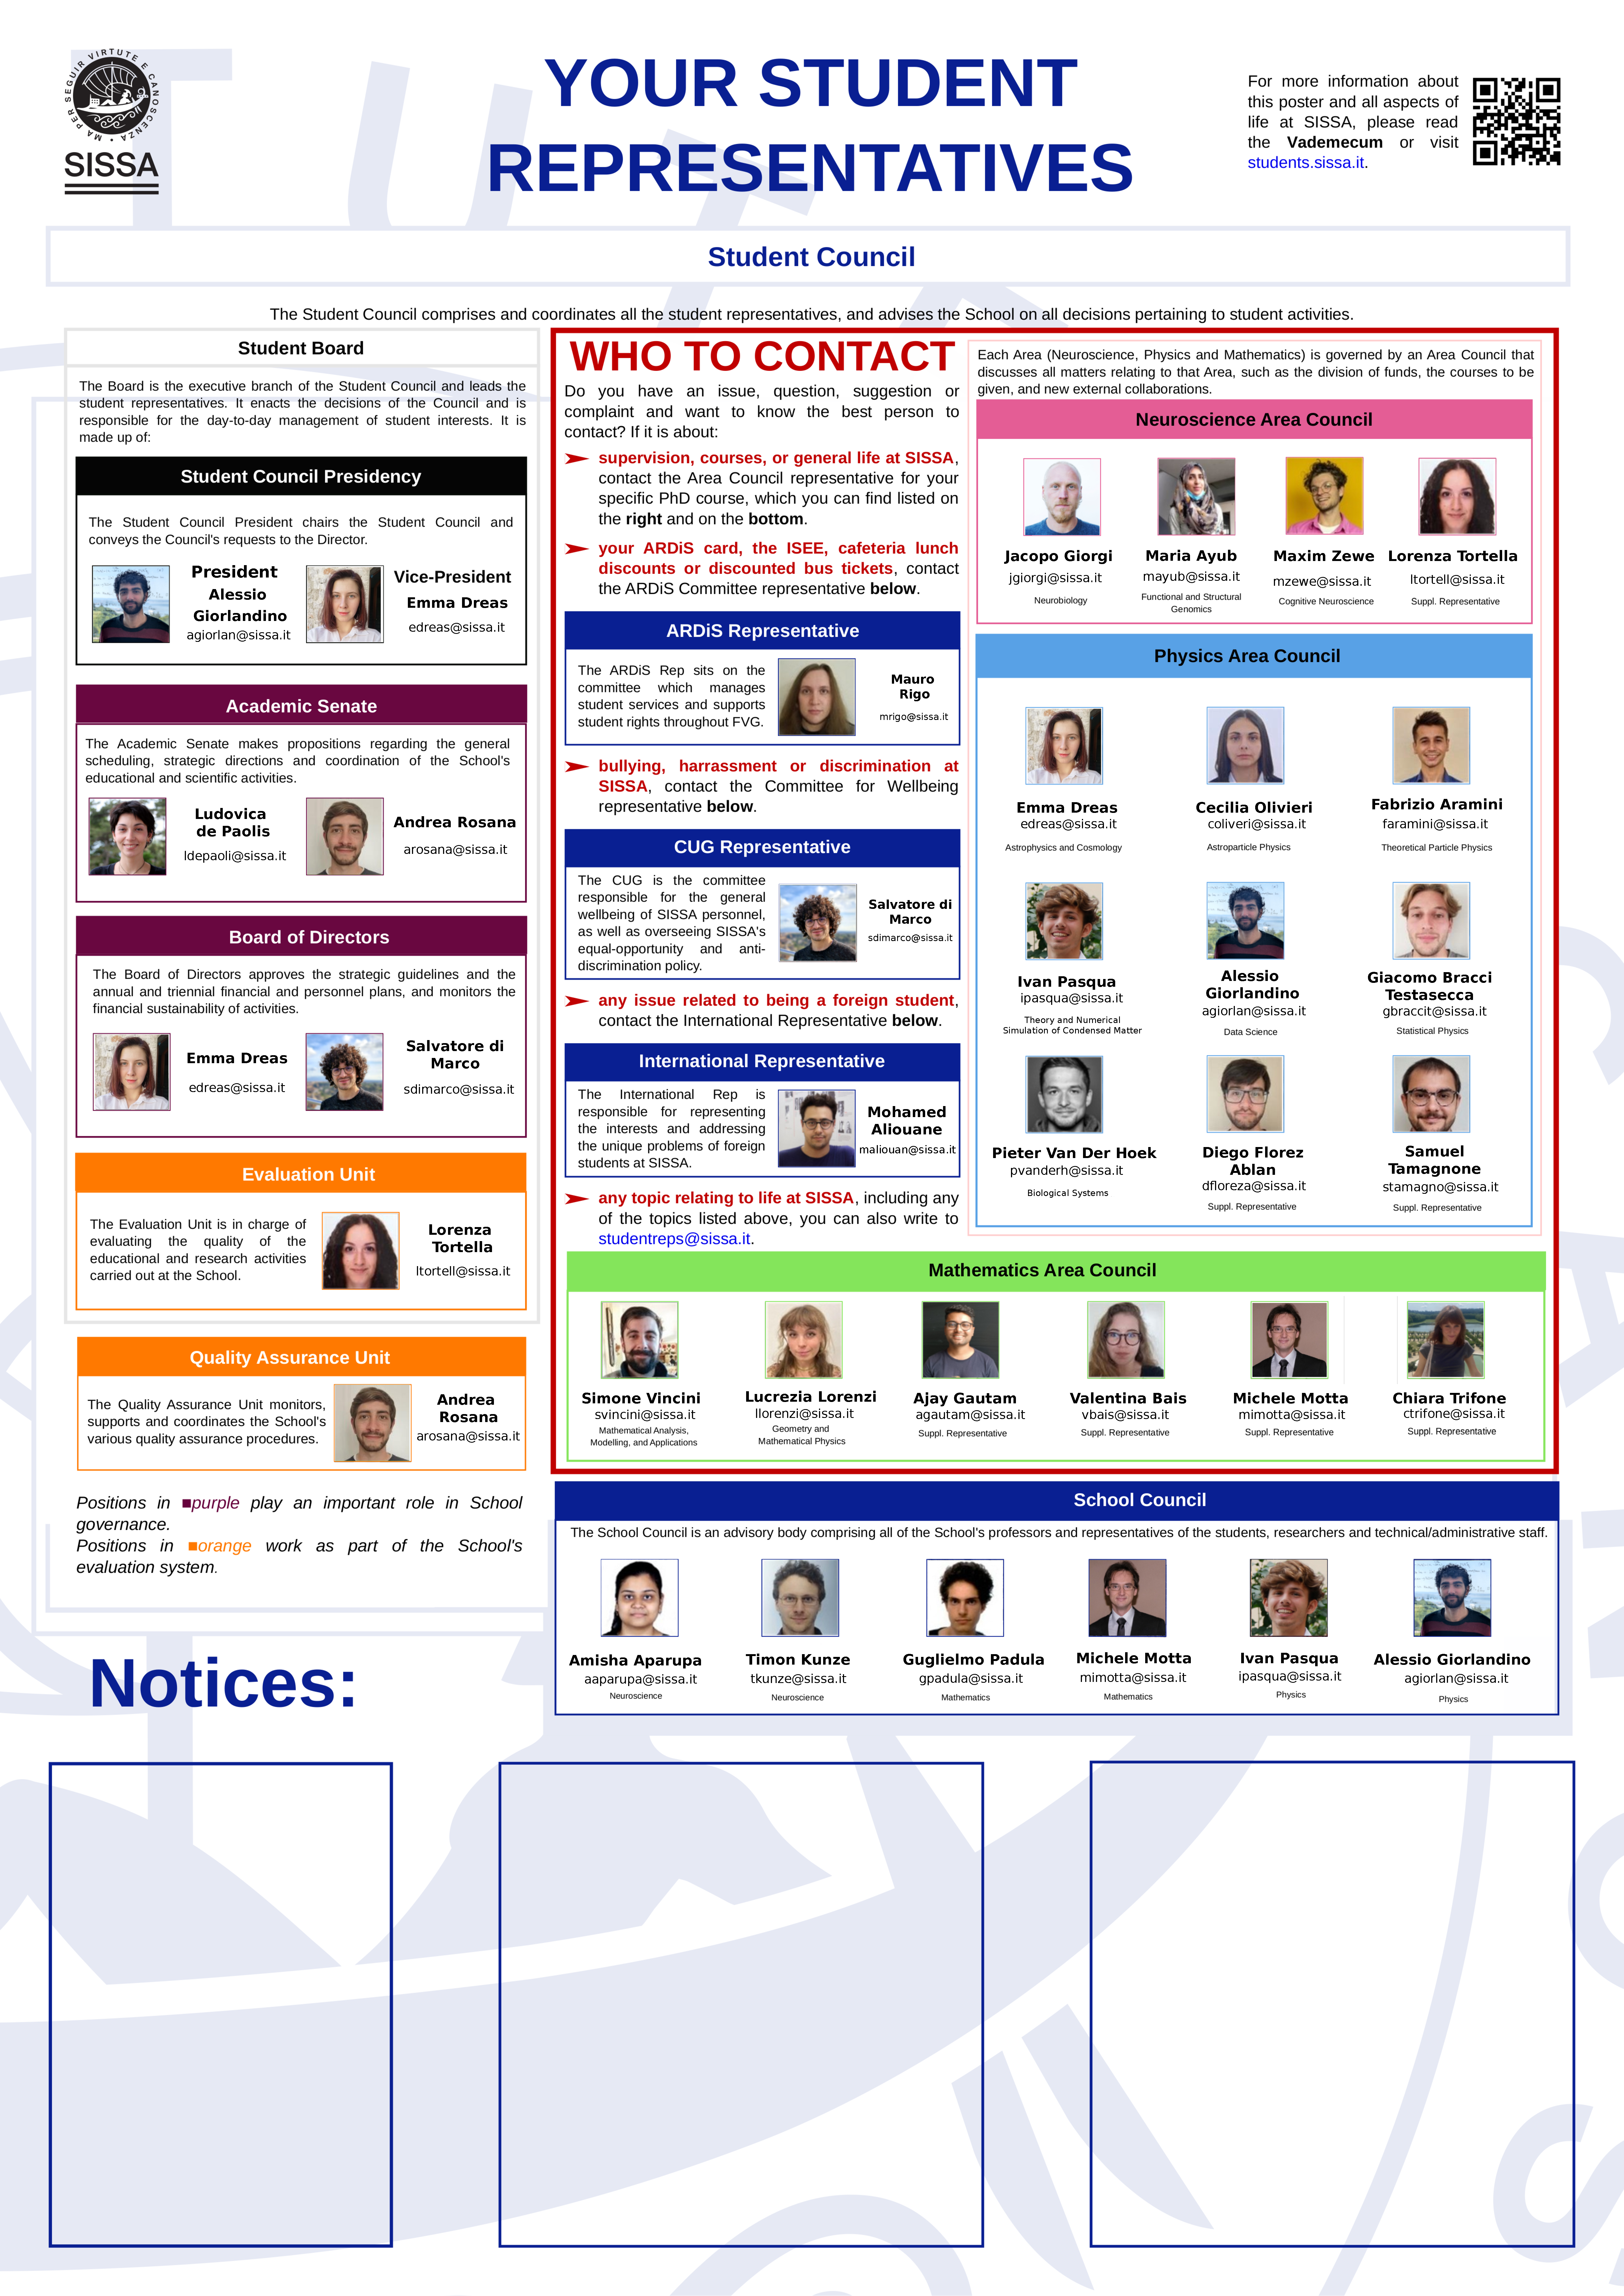
\includegraphics[scale = 1]{StudentPoster.pdf}	
\end{figure}
\restoregeometry


\chapter{Press Office (Media Relations and Communications Unit)}

The \textbf{SISSA Media Relations and Communications Unit} is in charge of managing media relations, social media and the SISSA website homepage. It takes care of preparing press releases, press reviews and the development of media products. Moreover, the Unit oversees the School's visual identity and organizes some of the School outreach events. If you are interested in promoting your research in the media, you are willing to take part in outreach initiatives or you have any enquiry concerning communication activities, please write to \linkemail{pressoffice@sissa.it} or contact any member of the \href{https://www.sissa.it/media-and-press}{Media Relations and Communications Unit}. Please also note that the SISSA logo, letterhead and PowerPoint templates are available at \href{https://www.sissa.it/researchers-and-sissa-staff}{this webpage}.


\chapter{Health and Safety Management}

\textbf{Health and Safety Management} is in charge of evaluating, communicating and preventing workplace hazards. In particular, among all the bureaucratic fulfillments that the School has to implement to guarantee its employers safety, this office is in charge of organizing the mandatory courses for first year student about health security (crucial above all in laboratories) and manage all kind of emergencies (fire, earthquakes, heart attacks, etc.) and possible buildings evacuation. If you need to contact
\begin{itemize}
	\item  a First Aid Operator urgently you can either call the \textcolor[rgb]{0.06666667,0.33333334,0.8}{911} from any internal SISSA phone or the 040-3787911 by your personal mobile phone. To report minor accidents and to notify the lack of necessary materials in First Aid Boxes, you can send an email to \linkemail{911@sissa.it}. 
	\item Emergency Evacuation/Fire Protection personnel urgently you can either call the \textcolor[rgb]{0.06666667,0.33333334,0.8}{555} from any internal SISSA phone or the 040-3787555 by your personal mobile phone. To report issues related to fire starting and situations that you feel abnormal or potentially dangerous (like a fire door that does not close well or by itself) you can send an email to \linkemail{555@sissa.it}. 
\end{itemize}
Remember that in both cases there are about 20 suitably trained people ready to help you. If there is any emergency, please do not call by your self the Italian Number for Emergencies (112), because if an ambulance comes here in SISSA and does not know where to go (there are several buildings and one of them is much bigger than the others) it will not be very useful. The right procedure consists instead in firstly contacting the internal number 911: a trained operator will come to give you support, while the other operators will call and welcome an ambulance at the entrance of SISSA (to bring First Aid Operators straightly where needed). Remember further that throughout the European Union the abuse or simply the joking call of these numbers is considered illegal by law. 

In SISSA there is a portable defibrillator that can be used only by authorized personnel. However, since people can enter the building also during the weekends when the First Aid surveillance is not present, it is good to know that it is installed at floor $0$ diametrically opposite with respect to the reception. NEVER TOUCH THE DEFIBRILLATOR IN ABSENCE OF AN EMERGENCY because it is alarmed and linked with the ambulance station. Any abuse will be pursued (there are cameras!). 

Remember also that if you want to bring from home some additional chairs, tables, electric boilers and so on, they have first to be approved by this office. For any other issue you can contact the Health and Safety Management at \linkemail{safety@sissa.it}. More info can be found on this \href{http://www.sissa.it/safety}{website}.

\chapter{Miscellaneous Contacts}

In addition to the contacts listed in the previous chapters, there are a number of contacts you may find very useful on occasion during your stay at SISSA. Some of the more commonly needed ones are listed in the table below for future reference.

\begin{center}
    \begin{tabular}{ l @{\hskip 4\tabcolsep} p{10.0cm} }
    \toprule
    \emph{\textbf{Address}} & \emph{\textbf{Contact them for \ldots}} \\ \midrule %\hline\hline
        \linkemail{phd@sissa.it} & \ldots submitting enquiries to the students secretariat \\
        \linkemail{helpdesk@sissa.it} & \ldots issues with software or hardware (workstations, phones, printers, etc.), borrowing laptops \\
        \linkemail{loandesk@sissa.it} & \ldots general library enquiries, book reservations, loan renewals \\
        \linkemail{phonebook@sissa.it} & \ldots requesting updates to or reporting errors in the \href{https://services.sissa.it/phonebook/}{SISSA Phonebook} \\
        \linkemail{plotter@sissa.it} & \ldots printing posters \\
        \linkemail{store@sissa.it} & \ldots requesting stationery items from the SISSA Store \\
        \linkemail{toner@sissa.it} & \ldots reporting when a printer has run out of ink \\
        \linkemail{valorisation@sissa.it} & \ldots enquiries related to knowledge transfer and research valorisation activities, such as the PhD4PMI and JOBFair programs \\
        \linkemail{ufficiotecnico@sissa.it} & \ldots general maintenance/repair requests \\
        \linkemail{911@sissa.it} & \ldots  reporting small accidents and notifying the lack of essential materials in the First Aid Boxes \\
        \linkemail{555@sissa.it} & \ldots reporting issues related to fire starting and situations that you feel abnormal or potentially dangerous (like a fire door that does not close well or by itself) \\
        \bottomrule
    \end{tabular}
\end{center}

	

\end{document}


%%%%%%%%%%%%%%%%%%%%%%%%%%%%%%%%%%%%%%%%%%%%%%%%%%%%%%%%%%%
%                                                         %
% *** END OF VADEMECUM.TEX ***                            %
%                                                         %
%%%%%%%%%%%%%%%%%%%%%%%%%%%%%%%%%%%%%%%%%%%%%%%%%%%%%%%%%%%
